\documentclass[11pt,a4paper,twocolumn]{article}

\usepackage[utf8]{inputenc}
\usepackage[T1]{fontenc}
\usepackage[spanish,es-tabla]{babel}
\usepackage[margin=1.7cm]{geometry}
\usepackage{graphicx}
\usepackage{float}
\usepackage{booktabs}
\usepackage{array}
\usepackage{tabularx}
\usepackage{hyperref}
\usepackage{setspace}
\usepackage{xcolor}
\usepackage{listings}
\usepackage{amsmath}
\usepackage{amssymb}
\usepackage{fancyhdr}
\usepackage{titlesec}
\usepackage{caption}
\usepackage{enumitem}
\usepackage{tikz}
\usetikzlibrary{shapes.geometric,arrows.meta,positioning,calc,fit,backgrounds}

\setstretch{1.08}
\hypersetup{colorlinks=true,linkcolor=black,urlcolor=blue,citecolor=blue}

\pagestyle{fancy}
\fancyhf{}
\fancyhead[L]{\small Práctica 3 -- Analítica de Datos}
\fancyhead[R]{\small Optimización de hiperparámetros -- Grupo 4}
\fancyfoot[C]{\thepage}
\renewcommand{\headrulewidth}{0.4pt}
\setlength{\headheight}{14.5pt}

\captionsetup[figure]{font=small,labelfont=bf}
\captionsetup[table]{font=small,labelfont=bf}

% Evita que LaTeX estire el espacio vertical para rellenar columnas (los
% "saltos" entre parrafos): el espacio sobrante se acumula al pie de la columna.
\raggedbottom

\titleformat{\section}{\normalfont\large\bfseries}{\thesection}{0.6em}{}
\titleformat{\subsection}{\normalfont\normalsize\bfseries}{\thesubsection}{0.5em}{}

\lstset{
  language=Python,
  basicstyle=\ttfamily\fontsize{7.4}{8.6}\selectfont,
  breaklines=true,
  frame=single,
  numbers=left,
  numberstyle=\tiny\color{gray},
  showstringspaces=false,
  keywordstyle=\color{blue!70!black},
  commentstyle=\color{green!50!black},
  stringstyle=\color{red!60!black},
  tabsize=2,
  xleftmargin=0.7em,
  framexleftmargin=0.7em,
  extendedchars=true,
  inputencoding=utf8,
  literate=
    {á}{{\'a}}1 {é}{{\'e}}1 {í}{{\'i}}1 {ó}{{\'o}}1 {ú}{{\'u}}1
    {Á}{{\'A}}1 {É}{{\'E}}1 {Í}{{\'I}}1 {Ó}{{\'O}}1 {Ú}{{\'U}}1
    {ñ}{{\~n}}1 {Ñ}{{\~N}}1
    {ü}{{\"u}}1,
}

\graphicspath{{figs/}}

% --- Valores reales de la corrida; los \providecommand de abajo solo actuan
%     como respaldo si numbers.tex no existe (no sobre-escriben) ---
\IfFileExists{numbers.tex}{\input{numbers.tex}}{}
\providecommand{\Nsamples}{60\,000}\providecommand{\Nfeatures}{22}
\providecommand{\Ntargets}{3}\providecommand{\Nclasses}{3}
\providecommand{\Searchsub}{12\,000}\providecommand{\CVfolds}{3}
\providecommand{\Ntrain}{48\,000}\providecommand{\Ntest}{12\,000}
\providecommand{\IRtargetone}{5.39}\providecommand{\IRtargettwo}{3.67}\providecommand{\IRtargetthree}{2.27}\providecommand{\IRmax}{5.39}
\providecommand{\GridCV}{0}\providecommand{\GridTime}{0}\providecommand{\GridEvals}{16}
\providecommand{\RandCV}{0}\providecommand{\RandTime}{0}\providecommand{\RandEvals}{25}
\providecommand{\OptunaCV}{0}\providecommand{\OptunaTime}{0}\providecommand{\OptunaTrials}{40}
\providecommand{\GenCV}{0}\providecommand{\GenTime}{0}\providecommand{\GenEvals}{0}\providecommand{\GenPop}{16}\providecommand{\GenGen}{6}
\providecommand{\GridFtest}{0}\providecommand{\GridGap}{0}\providecommand{\GridHam}{0}\providecommand{\GridSubset}{0}
\providecommand{\RandFtest}{0}\providecommand{\RandGap}{0}\providecommand{\RandHam}{0}\providecommand{\RandSubset}{0}
\providecommand{\OptunaFtest}{0}\providecommand{\OptunaGap}{0}\providecommand{\OptunaHam}{0}\providecommand{\OptunaSubset}{0}
\providecommand{\GenFtest}{0}\providecommand{\GenGap}{0}\providecommand{\GenHam}{0}\providecommand{\GenSubset}{0}
\providecommand{\BestOpt}{Optuna (Bayes)}\providecommand{\BestOptF}{0}
\providecommand{\OptunaAlgo}{random\_forest}\providecommand{\GenAlgo}{logistic}\providecommand{\TotalRuntime}{0}
\providecommand{\PARF}{0}\providecommand{\PADT}{0}\providecommand{\PAMLP}{0}\providecommand{\PANB}{0}\providecommand{\PALR}{0}
\providecommand{\BestAlgo}{random\_forest}\providecommand{\BestAlgoF}{0}\providecommand{\WorstAlgo}{decision\_tree}\providecommand{\WorstAlgoF}{0}
\providecommand{\LCgap}{0}\providecommand{\LCtrainEnd}{0}\providecommand{\LCcvEnd}{0}\providecommand{\LCcvStart}{0}\providecommand{\PCAneff}{16}
\providecommand{\BaseF}{0}\providecommand{\RecOneF}{0}\providecommand{\RecOneDelta}{0}\providecommand{\RecOneViable}{viable}
\providecommand{\RecTwoF}{0}\providecommand{\RecTwoDelta}{0}\providecommand{\RecTwoComp}{16}\providecommand{\RecTwoViable}{no viable}
\providecommand{\RecThreeF}{0}\providecommand{\RecThreeDelta}{0}\providecommand{\RecThreeViable}{no viable}
\providecommand{\TablaDist}{target1 & 61 & 27 & 11 & 5 \\}
\providecommand{\TablaOptim}{Grid & 0 & 0 & 0 & 0 & 0 & 0 \\}
\providecommand{\TablaRec}{Baseline & 0 & 0 & 0 & -- \\}

\begin{document}

%==========================================================
% CARÁTULA
%==========================================================
\onecolumn
\begin{titlepage}
\centering
\vspace*{0.4cm}
{\large \textbf{UNIVERSIDAD NACIONAL DE INGENIERÍA}}\\[0.15cm]
{\normalsize FACULTAD DE INGENIERÍA INDUSTRIAL Y DE SISTEMAS}

\vspace{0.7cm}
\includegraphics[width=3.6cm]{uni.png}

\vspace{0.9cm}
{\LARGE \textbf{PRÁCTICA 3}}

\vspace{0.3cm}
{\Large Optimización automática de hiperparámetros\\
para un modelo de clasificación multi-target\\
desbalanceado con Scikit-Learn}

\vspace{1.3cm}
\begin{tabular}{rl}
\textbf{Curso}     & : Analítica de Datos (SI150V / ST150V) \\
\textbf{Docente}   & : Samuel Alonso Oporto Díaz \\
\textbf{Grupo}     & : 4 \\
\textbf{Fecha}     & : 8 de junio del 2026 \\
\end{tabular}

\vspace{1.0cm}
\textbf{Integrantes}\\[0.25cm]
\begin{tabular}{lll}
De la Cruz Orellana, Aleksander     & 20212099E & \\
León Sánchez, Fransua Mijail        & 20210019D & \\
López Arana, Edgar Michael          & 20210254C & \\
\end{tabular}

\vspace{0.9cm}
\textbf{Repositorio de código}\\[0.2cm]
\url{https://drive.google.com/drive/folders/1p4MXPYVENPGY_9TKOuh8KOs5D-tUMGOD?usp=drive_link}

\vfill
LIMA -- PERÚ\\
2026
\end{titlepage}

%==========================================================
% RESUMEN
%==========================================================
\twocolumn
\section*{Resumen}
Se construyó un procedimiento de aprendizaje automático cuyo objetivo es minimizar el error de
clasificación sobre un problema \textit{multi-target} (tres variables objetivo, cada una con tres clases)
generado sintéticamente con \texttt{scikit-learn}: \Nsamples{} registros, \Nfeatures{} atributos y una
distribución de clases deliberadamente desbalanceada (razón mayoritaria/minoritaria de hasta \IRmax{}). El
núcleo del trabajo no es un único modelo, sino el \emph{algoritmo de optimización} que calcula
automáticamente sus parámetros: se implementaron y compararon cuatro estrategias de búsqueda de
hiperparámetros ---búsqueda en cuadrícula (\textit{Grid Search}), búsqueda aleatoria (\textit{Random
Search}), optimización bayesiana (Optuna/TPE) y un algoritmo genético (DEAP)--- evaluadas con validación
cruzada de \CVfolds{} pliegues y la métrica F1-macro promediada sobre los tres \textit{targets}. Los dos
optimizadores que además buscan sobre la \emph{elección del algoritmo} (Optuna y el genético) prácticamente
empataron en el tope ---F1-macro de \OptunaFtest{} y \GenFtest{} en prueba--- y ambos seleccionaron la red
neuronal (MLP) como mejor algoritmo de aprendizaje entre los cinco evaluados (redes neuronales, árbol de
decisión, \textit{random forest}, \textit{naive bayes} y regresión logística), superando ampliamente a la
cuadrícula y la búsqueda aleatoria (\GridFtest{} y \RandFtest{}), que quedaron limitadas a un solo modelo.
La optimización bayesiana resultó la más \emph{eficiente} (igual calidad en \OptunaTime{}~s frente a
\GenTime{}~s del genético). El análisis de la curva de
aprendizaje confirmó que el problema es propenso al sobreaprendizaje cuando se libera la profundidad del
modelo (brecha entrenamiento--validación de \LCgap{}), y de las tres recomendaciones implementadas la
ponderación de clases (\texttt{class\_weight=balanced}) fue la única que mejoró la métrica sobre la línea
base (\RecOneDelta{}), demostrando ser \RecOneViable{}.

\vspace{0.3em}
\noindent\textbf{Palabras clave:} optimización de hiperparámetros, clasificación multi-target,
desbalanceo, F1-macro, Grid Search, Random Search, optimización bayesiana, algoritmo genético, MLOps,
Scikit-Learn.

%==========================================================
% 1. INTRODUCCIÓN
%==========================================================
\section{Introducción}
El rendimiento de un modelo de aprendizaje supervisado depende tanto de los parámetros que se ajustan
durante el entrenamiento (pesos, umbrales, particiones del árbol) como de los \emph{hiperparámetros} que el
analista fija antes de entrenar: la profundidad de un árbol, el número de neuronas de una red o la fuerza
de regularización. Estos últimos no se aprenden por descenso del gradiente ni por el criterio de impureza;
deben buscarse en un espacio de configuraciones que crece de forma combinatoria. El problema de
\emph{calcular automáticamente} esos hiperparámetros es lo que la literatura denomina \textit{Hyperparameter
Optimization} (HPO) y constituye el corazón de esta práctica~\cite{feurer2019,bergstra2012}.

\textbf{Antecedentes.} La forma más antigua de HPO es la búsqueda en cuadrícula, que evalúa de manera
exhaustiva todas las combinaciones de una rejilla discreta. Bergstra y Bengio~\cite{bergstra2012}
demostraron empíricamente que, cuando solo unas pocas dimensiones son relevantes, la búsqueda aleatoria
encuentra mejores configuraciones que la cuadrícula con el mismo presupuesto, porque no desperdicia
evaluaciones sobre dimensiones irrelevantes. Posteriormente, los métodos secuenciales basados en modelos
---la optimización bayesiana--- propusieron \emph{aprender} de las evaluaciones anteriores para decidir la
siguiente, mediante un modelo sustituto y una función de adquisición~\cite{shahriari2016}. El estimador de
Parzen estructurado en árbol (TPE) que implementa Optuna~\cite{akiba2019} pertenece a esta familia. En
paralelo, los algoritmos evolutivos abordan el mismo problema como una optimización poblacional inspirada en
la selección natural~\cite{goldberg1989}. Todas estas técnicas conviven hoy en frameworks de AutoML y de
MLOps.

\textbf{Procedimiento.} En este trabajo (i)~se genera un conjunto de datos multi-target desbalanceado con
Scikit-Learn~\cite{geron2019}; (ii)~se define un espacio de búsqueda que abarca no solo los hiperparámetros
de cada algoritmo de aprendizaje sino también las decisiones de preprocesamiento (normalización, reducción
de dimensionalidad, ponderación de clases) y la elección misma del algoritmo; (iii)~se implementan cuatro
optimizadores sobre ese espacio; y (iv)~se selecciona la mejor configuración y se la somete a un análisis de
sobreaprendizaje y a la implementación de recomendaciones.

\textbf{Resultados esperados.} Se espera que la búsqueda aleatoria y la bayesiana superen a la cuadrícula en
relación calidad/tiempo, que la métrica F1-macro sea sensible al desbalanceo y que el modelo presente
sobreaprendizaje al aumentar su capacidad, lo cual justifica el uso de regularización y ponderación de
clases como contramedidas.

%==========================================================
% 2. PLANTEAMIENTO DEL PROBLEMA
%==========================================================
\section{Planteamiento del problema}
\subsection{Sistematización de conceptos}
El enunciado fija un vocabulario preciso que conviene formalizar. Un \textbf{target} es una variable que el
modelo debe predecir (una columna de la matriz de salida). El \textbf{conjunto de clases} de un target es el
conjunto de todos sus valores posibles; una \textbf{clase} es uno de esos valores asignado a una instancia
(también llamado \emph{estado}), y una \textbf{etiqueta} (\textit{label}) es la clase concreta observada en
una instancia particular. Con estas definiciones, la Figura~\ref{fig:tipos} resume los cuatro tipos de
problema de clasificación: binario (un target, dos clases), multiclase (un target, $>2$ clases),
multietiqueta (varios labels binarios simultáneos) y multi-target o \textit{multi-output} (varios targets,
cada uno con su propio conjunto de clases, predichos conjuntamente).

\begin{figure}[H]
\centering
\includegraphics[width=\columnwidth]{tipos_clasificacion.png}
\caption{Tipos de problema de clasificación según el número de \textit{targets} y de clases por
\textit{target}. Nuestro caso corresponde a la cuarta categoría: multi-target con tres clases por
\textit{target}.}
\label{fig:tipos}
\end{figure}

\subsection{El problema concreto y la decisión sobre los datos}
El enunciado pide datos con ``al menos 3 labels, al menos 3 clases por cada label, al menos 20 atributos y
al menos 50\,000 registros'', desbalanceados, generados con \texttt{make\_multilabel\_classification()} o,
alternativamente, con \texttt{make\_classification()}. Existe una incompatibilidad técnica que debe
explicitarse: \texttt{make\_multilabel\_classification} produce \emph{labels binarios} (presencia/ausencia),
de modo que cada \textit{label} tendría solo dos clases y nunca tres. Por ello, para satisfacer
literalmente el requisito de ``$\geq 3$ clases por \textit{label}'' se utilizó la alternativa explícita del
enunciado, \texttt{make\_classification()}, para construir un problema \textbf{multi-target multiclase}:
$T=\Ntargets{}$ targets, cada uno con $K=\Nclasses{}$ clases, sobre una misma matriz de
$\Nfeatures{}$ atributos y $\Nsamples{}$ registros. No obstante, para no descartar la función nombrada en
primer lugar, también se generó el conjunto multietiqueta y se reprodujeron con datos reales las tablas de
contingencia de frecuencias que el enunciado presenta como ejemplo (Sección~\ref{sec:c1}).

\subsection{Formalización}
Sea $\mathbf{x}\in\mathbb{R}^{\Nfeatures{}}$ el vector de atributos de una instancia y
$\mathbf{y}=(y^{(1)},\dots,y^{(T)})$ su vector de etiquetas, con $y^{(t)}\in\{0,1,2\}$. Se busca una función
$f_\lambda:\mathbb{R}^{\Nfeatures{}}\!\to\!\{0,1,2\}^{T}$, parametrizada por una configuración de
hiperparámetros $\lambda$, que minimice el error esperado:
\begin{equation}
\lambda^\star=\arg\min_{\lambda\in\Lambda}\;\mathbb{E}_{(\mathbf{x},\mathbf{y})}\!\big[\mathcal{L}(\mathbf{y},f_\lambda(\mathbf{x}))\big],
\label{eq:obj}
\end{equation}
donde $\Lambda$ es el espacio de búsqueda y $\mathcal{L}$ una pérdida de clasificación. Como
$\mathbb{E}[\cdot]$ es desconocida, se la aproxima con el promedio de la métrica sobre validación cruzada
(Sección~\ref{sec:metrica}). La Ecuación~\eqref{eq:obj} encierra los \emph{dos} objetivos integrados que
señala el enunciado: el objetivo de aprendizaje (minimizar el error de $f$) y el objetivo de optimización
(encontrar el $\lambda$ que lo minimiza).

%==========================================================
% 3. METODOLOGÍA
%==========================================================
\section{Metodología}
El proyecto se organizó siguiendo el modelo de referencia \textbf{MLOps}, adaptado a las fases que
realmente se desarrollan en esta práctica (no se incluyen despliegue en producción ni monitoreo en línea
porque exceden el alcance del entregable). La Figura~\ref{fig:mlops} muestra el ciclo adoptado: ingesta y
generación de datos, validación y análisis exploratorio, preparación, definición del espacio de búsqueda,
optimización de hiperparámetros (la pieza central), evaluación y, finalmente, empaquetado del modelo y de
los artefactos reproducibles.

\begin{figure}[H]
\centering
\begin{tikzpicture}[node distance=2.6mm and 4mm,
  every node/.style={font=\scriptsize},
  stage/.style={draw,rounded corners,fill=blue!8,minimum width=2.05cm,minimum height=0.7cm,align=center},
  arr/.style={-{Latex[length=1.6mm]},thick}]
\node[stage] (a) {Generación\\de datos};
\node[stage,right=of a] (b) {Validación\\y EDA};
\node[stage,right=of b] (c) {Preparación};
\node[stage,below=of c] (d) {Espacio de\\búsqueda};
\node[stage,left=of d] (e) {\textbf{Optimización}\\\textbf{(HPO)}};
\node[stage,left=of e] (f) {Evaluación};
\node[stage,below=14mm of f] (g) {Empaquetado\\reproducible};
\draw[arr] (a)--(b); \draw[arr] (b)--(c); \draw[arr] (c)--(d);
\draw[arr] (d)--(e); \draw[arr] (e)--(f); \draw[arr] (f)--(g);
% realimentacion evaluacion -> optimizacion, en U por debajo de las cajas
\draw[arr,dashed] (f.south) to[out=-90,in=-90,looseness=1.7] (e.south);
\node[font=\scriptsize\itshape] at ($(f.south)!0.5!(e.south)+(0,-0.6)$) {reajuste};
\end{tikzpicture}
\caption{Ciclo MLOps adaptado al proyecto. La optimización de hiperparámetros realimenta a la evaluación
hasta converger en la mejor configuración.}
\label{fig:mlops}
\end{figure}

Cada fase del ciclo se materializa en un \emph{componente} de software (Sección~\ref{sec:construccion}). La
trazabilidad se garantiza con una semilla aleatoria fija, el guardado de los datasets y predicciones en
\texttt{CSV}, y la exportación de todas las métricas a un archivo \texttt{results.json} del que se derivan
automáticamente las cifras de este informe.

%==========================================================
% 4. OBJETIVOS
%==========================================================
\section{Objetivos}
\textbf{Objetivo general.} Construir un procedimiento de aprendizaje que minimice el error de clasificación
multi-target mediante un algoritmo de optimización que calcule automáticamente los hiperparámetros del
modelo.

\noindent\textbf{Objetivos específicos (componentes).} Cada objetivo específico es un componente con
insumos y resultados bien definidos (Figura~\ref{fig:objetivos}):
\begin{enumerate}[leftmargin=1.1em,itemsep=1pt]
\item Generar un dataset multi-target desbalanceado que cumpla las restricciones del enunciado.
\item Preparar los datos y definir una métrica adecuada al desbalanceo.
\item Implementar y explicar los cuatro algoritmos de optimización sobre un espacio de búsqueda común.
\item Comparar los optimizadores y seleccionar la mejor configuración (modelo + preprocesamiento).
\item Diagnosticar el sobreaprendizaje y proponer e implementar recomendaciones.
\end{enumerate}

\begin{figure}[H]
\centering
\begin{tikzpicture}[node distance=3.5mm,every node/.style={font=\scriptsize},
  obj/.style={draw,rounded corners,fill=orange!12,minimum width=5.2cm,minimum height=0.52cm,align=center},
  io/.style={draw,rounded corners,fill=blue!8,minimum width=5.2cm,minimum height=0.52cm,align=center,font=\scriptsize\itshape},
  arr/.style={-{Latex[length=1.6mm]}}]
\node[io] (in) {insumos: atributos $\mathbf{x}$ y \textit{targets} $\mathbf{y}$};
\node[obj,below=of in] (o1) {O1--O2: generación de datos + métrica};
\node[obj,below=of o1] (o2) {O3: optimización de hiperparámetros};
\node[obj,below=of o2] (o4) {O4--O5: selección + diagnóstico};
\node[io,below=of o4] (out) {resultados: $\lambda^\star$, modelo y métricas};
\draw[arr] (in)--(o1);
\draw[arr] (o1)--node[right,font=\tiny]{$D,\,\mathcal{S}$}(o2);
\draw[arr] (o2)--(o4); \draw[arr] (o4)--(out);
\end{tikzpicture}
\caption{Encadenamiento de objetivos como componentes. El flujo entra por los insumos (arriba), atraviesa
cada objetivo --una caja por componente-- y entrega los resultados (abajo) que alimentan al siguiente.}
\label{fig:objetivos}
\end{figure}

%==========================================================
% 5. ARQUITECTURA
%==========================================================
\section{Arquitectura del sistema}
Se describe la arquitectura en tres niveles de detalle crecientes.

\begin{figure*}[!t]
\centering
\resizebox{0.86\textwidth}{!}{%
\begin{tikzpicture}[every node/.style={font=\small},
  box/.style={draw,very thick,rounded corners,fill=green!12,minimum width=5cm,minimum height=1.5cm,align=center},
  io/.style={draw,fill=blue!8,rounded corners,minimum width=3.1cm,minimum height=1.1cm,align=center},
  arr/.style={-{Latex[length=2.5mm]},very thick}]
\node[io] (in) {\textbf{Entrada}\\Dataset multi-target\\$\Nsamples{}\times\Nfeatures{}$, desbalanceado};
\node[box,right=1.8cm of in] (sys) {\textbf{Sistema de aprendizaje}\\\textbf{con optimización automática}\\de hiperparámetros};
\node[io,right=1.8cm of sys] (out) {\textbf{Salida}\\Modelo óptimo $f_{\lambda^\star}$\\+ predicciones $\hat{\mathbf{y}}$ + métricas};
\draw[arr] (in)--(sys); \draw[arr] (sys)--(out);
\end{tikzpicture}}
\caption{Arquitectura de \textbf{Nivel 0} (caja negra). El sistema recibe el dataset desbalanceado y
entrega el modelo óptimo, sus predicciones y sus métricas de desempeño.}
\label{fig:n0}
\end{figure*}

\begin{figure*}[!t]
\centering
\resizebox{\textwidth}{!}{%
\begin{tikzpicture}[node distance=8mm,every node/.style={font=\footnotesize},
  comp/.style={draw,rounded corners,fill=green!10,minimum width=2.3cm,minimum height=1cm,align=center},
  io/.style={draw,fill=blue!8,rounded corners,minimum width=1.9cm,minimum height=0.9cm,align=center},
  arr/.style={-{Latex[length=2mm]},thick}]
\node[io] (in) {Entrada\\(datos)};
\node[comp,right=of in] (c1) {C1\\Generación};
\node[comp,right=of c1] (c2) {C2\\Preparación};
\node[comp,right=of c2] (c3) {C3\\Espacio +\\métrica};
\node[comp,right=of c3] (c4) {C4--C7\\Optimizadores};
\node[comp,right=of c4] (c8) {C8\\Selección};
\node[io,right=of c8] (out) {Salida\\(modelo)};
\draw[arr] (in)--(c1);\draw[arr] (c1)--(c2);\draw[arr] (c2)--(c3);
\draw[arr] (c3)--(c4);\draw[arr] (c4)--(c8);\draw[arr] (c8)--(out);
\node[comp,below=1.1cm of c4] (c9) {C9\\Diagnóstico};
\draw[arr] (c8) |- (c9); \draw[arr,dashed] (c9) -| (c4);
\end{tikzpicture}}
\caption{Arquitectura de \textbf{Nivel 1}. La caja negra se abre en la cadena de componentes del
\textit{pipeline}; cada componente deja un artefacto persistente (CSV/PNG/JSON) que alimenta al siguiente.}
\label{fig:n1}
\end{figure*}

\begin{figure*}[!t]
\centering
\resizebox{\textwidth}{!}{%
\begin{tikzpicture}[node distance=5mm and 7mm,every node/.style={font=\scriptsize},
  comp/.style={draw,rounded corners,fill=green!10,minimum width=2.1cm,minimum height=0.7cm,align=center},
  sub/.style={draw,dashed,rounded corners,fill=yellow!12,minimum width=2.0cm,minimum height=0.55cm,align=center},
  arr/.style={-{Latex[length=1.5mm]}}]
\node[comp] (c4) {C4 Grid};
\node[comp,right=of c4] (c5) {C5 Random};
\node[comp,right=of c5] (c6) {C6 Optuna};
\node[comp,right=of c6] (c7) {C7 Genético};
\node[sub,below=of c4] (s4) {rejilla\\exhaustiva};
\node[sub,below=of c5] (s5) {muestreo\\aleatorio};
\node[sub,below=of c6] (s6) {modelo TPE\\+ adquisición};
\node[sub,below=of c7] (s7) {población\\+ cruce/mutación};
\draw[arr] (c4)--(s4);\draw[arr] (c5)--(s5);\draw[arr] (c6)--(s6);\draw[arr] (c7)--(s7);
\node[comp,fill=blue!10,below=1.0cm of s5,xshift=1cm,minimum width=4.6cm] (cv) {Validación cruzada $\CVfolds{}$-fold con F1-macro sobre Pipeline(preproceso + modelo)};
\draw[arr] (s4)--(cv);\draw[arr] (s5)--(cv);\draw[arr] (s6)--(cv);\draw[arr] (s7)--(cv);
\end{tikzpicture}}
\caption{Arquitectura de \textbf{Nivel 2}. Detalle de los sub-procedimientos de cada optimizador; todos
comparten el mismo evaluador: validación cruzada con F1-macro sobre un \textit{pipeline} que encadena
preprocesamiento y modelo.}
\label{fig:n2}
\end{figure*}

%==========================================================
% 6. CONSTRUCCIÓN DE LOS COMPONENTES
%==========================================================
\section{Construcción de los componentes}
\label{sec:construccion}
Cada componente se presenta con un fragmento del código fuente real, el resultado de su corrida y la
explicación de lo realizado. El código completo se entrega comprimido junto al informe.

\subsection{C1. Generación del dataset}
\label{sec:c1}
El \textit{target} 1 se generó directamente con \texttt{make\_classification} (tres clases con pesos
$0.62/0.27/0.11$). Los \textit{targets} 2 y 3 se construyeron como funciones ---una de ellas no lineal---
de las doce primeras variables informativas, discretizadas por cuantiles para inducir desbalanceo. Así los
tres \textit{targets} dependen genuinamente de los mismos atributos y son aprendibles.

\begin{lstlisting}[caption={C1 -- Generación multi-target multiclase desbalanceada}]
X, y1 = make_classification(
    n_samples=60000, n_features=22, n_informative=12,
    n_redundant=4, n_classes=3, n_clusters_per_class=2,
    weights=[0.62, 0.27, 0.11], class_sep=0.9,
    flip_y=0.02, shuffle=False, random_state=SEED)

inf = X[:, :12]
def build_target(seed, cuts, nonlin=False):
    w = np.random.RandomState(seed).randn(inf.shape[1])
    score = inf @ w
    if nonlin:
        score += 0.6*(inf[:,0]*inf[:,3]) - 0.5*(inf[:,5]**2)
    score += rng.normal(0, score.std()*0.35, len(score))
    return np.digitize(score, np.quantile(score, cuts))

y2 = build_target(101, [0.55, 0.85], nonlin=True)
y3 = build_target(202, [0.50, 0.78])
Y = np.column_stack([y1, y2, y3])
\end{lstlisting}

La Tabla~\ref{tab:dist} y la Figura~\ref{fig:dist} confirman el desbalanceo buscado: la clase mayoritaria
del \textit{target} 1 es \IRtargetone{} veces más frecuente que la minoritaria. Este desbalanceo es lo que
obliga a elegir una métrica robusta (Sección~\ref{sec:metrica}).

El diseño se comprobó con tres pruebas de variedad. Primero, las \textbf{27} combinaciones posibles de
$(y^{(1)},y^{(2)},y^{(3)})$ aparecen en los datos (la menos frecuente con 204 instancias), de modo que no
hay estados degenerados. Segundo, los tres \textit{targets} son casi \textbf{independientes} entre sí
(información mutua normalizada inferior a $0.003$): cada uno es un problema de predicción distinto y no una
copia de otro. Tercero, cada \textit{target} se apoya en un \textbf{subconjunto diferente} de atributos ---la
información mutua máxima atributo-objetivo va de $0.06$ a $0.16$ según el \textit{target}---, lo que evita un
dataset trivial y mantiene el problema genuinamente multivariado.

\begin{table}[H]
\centering
\caption{Distribución de clases por \textit{target} (\% de registros) y razón de desbalanceo (RD).}
\label{tab:dist}
\small
\begin{tabular}{lcccc}
\toprule
\textbf{Target} & \textbf{clase 0} & \textbf{clase 1} & \textbf{clase 2} & \textbf{RD} \\
\midrule
\TablaDist
\bottomrule
\end{tabular}
\end{table}

\begin{figure}[H]
\centering
\includegraphics[width=\columnwidth]{fig_class_dist.png}
\caption{Distribución de frecuencias de clase por \textit{target}. Las barras evidencian la asimetría
(clase 0 dominante) que caracteriza a un problema desbalanceado.}
\label{fig:dist}
\end{figure}

Adicionalmente, con \texttt{make\_multilabel\_classification} se reprodujo el ejemplo de tablas de
contingencia del enunciado. La Figura~\ref{fig:cont} muestra la co-ocurrencia real de \texttt{label1} y
\texttt{label2}: la celda $(1,1)$ concentra la mayor masa de probabilidad, exactamente el patrón de
desbalanceo conjunto que ilustra el enunciado.

\begin{figure}[H]
\centering
\includegraphics[width=0.78\columnwidth]{fig_contingency.png}
\caption{Tabla de contingencia \texttt{label1}$\times$\texttt{label2} (\% del total) obtenida con
\texttt{make\_multilabel\_classification}, réplica con datos reales del ejemplo del enunciado.}
\label{fig:cont}
\end{figure}

\subsection{C2. Preparación de datos}
Se dividió el conjunto en \Ntrain{} registros de entrenamiento y \Ntest{} de prueba (80/20). Para acelerar
la \emph{fase de búsqueda} ---que repite cientos de ajustes--- se trabajó sobre una submuestra de
\Searchsub{} registros; el modelo ganador se reajusta luego sobre el entrenamiento completo. El propio
tamaño de la muestra de entrenamiento es, de hecho, uno de los parámetros del proceso de aprendizaje que el
enunciado pide considerar, y su efecto se cuantifica en la curva de aprendizaje (Sección~\ref{sec:c9}). La
normalización (\texttt{StandardScaler}/\texttt{MinMaxScaler}/ninguna) no se fija a priori sino que se
incorpora como una decisión más del espacio de búsqueda.

\subsection{C3. Espacio de búsqueda y métrica}
\label{sec:metrica}
\textbf{Métrica.} Con clases desbalanceadas, la exactitud (\textit{accuracy}) es engañosa: un clasificador
que prediga siempre la clase mayoritaria del \textit{target}~1 lograría $\approx$61\% de aciertos sin
aprender nada. Por eso se adopta el \textbf{F1-macro}, media no ponderada del F1 de cada clase, que penaliza
el mal desempeño en clases minoritarias. Para el caso multi-target se promedia además sobre los $T$ targets:
\begin{equation}
\text{F1}_{\text{macro}}=\frac{1}{T}\sum_{t=1}^{T}\frac{1}{K}\sum_{k=1}^{K}\frac{2\,P^{(t)}_k R^{(t)}_k}{P^{(t)}_k+R^{(t)}_k},
\label{eq:f1}
\end{equation}
donde $P$ y $R$ son precisión y \textit{recall}. Se reportan también la \emph{Hamming loss} (fracción de
etiquetas mal predichas) y la \emph{subset accuracy} (aciertan los tres \textit{targets} a la vez). Toda la
evaluación se realiza con validación cruzada de Scikit-Learn.\footnote{\scriptsize\url{https://scikit-learn.org/1.4/tutorial/statistical_inference/model_selection.html}}

\begin{lstlisting}[caption={C3 -- Métrica F1-macro multi-target como scorer de Scikit-Learn}]
def f1_macro_multioutput(y_true, y_pred):
    return np.mean([
        f1_score(y_true[:, j], y_pred[:, j], average="macro")
        for j in range(y_true.shape[1])])

SCORER = make_scorer(f1_macro_multioutput)
\end{lstlisting}

\textbf{Espacio de búsqueda.} El espacio $\Lambda$ es un \textit{pipeline} configurable que recoge los
parámetros del proceso de aprendizaje que enumera el enunciado: el \emph{tamaño de la muestra de
entrenamiento} (Sección~\ref{sec:c9}), la \emph{técnica de normalización} (escalador estándar, min-max o
ninguno), el \emph{número de atributos} que entran al modelo (vía PCA), el \emph{balanceo de clases} por
\textit{target} (\texttt{class\_weight}), la \emph{elección del algoritmo} de aprendizaje entre los cinco
solicitados y los \emph{hiperparámetros} propios de cada uno (Tabla~\ref{tab:hp}). Los algoritmos sin
soporte multi-target nativo (\textit{naive bayes}, regresión logística) se envuelven en
\texttt{MultiOutputClassifier}, que ajusta un estimador independiente por \textit{target}.

\begin{table}[H]
\centering
\caption{Hiperparámetros optimizados por algoritmo de aprendizaje.}
\label{tab:hp}
\scriptsize
\begin{tabularx}{\columnwidth}{lX}
\toprule
\textbf{Algoritmo} & \textbf{Hiperparámetros} \\
\midrule
Random Forest & \texttt{n\_estimators}, \texttt{max\_depth}, \texttt{min\_samples\_split}, \texttt{max\_features}, \texttt{class\_weight} \\
Árbol decisión & \texttt{max\_depth}, \texttt{min\_samples\_split}, \texttt{min\_samples\_leaf}, \texttt{criterion}, \texttt{class\_weight} \\
Red neuronal (MLP) & \texttt{hidden\_layer\_sizes}, \texttt{activation}, \texttt{alpha}, \texttt{learning\_rate\_init} \\
Naive Bayes & \texttt{var\_smoothing} \\
Reg. logística & \texttt{C}, \texttt{class\_weight} \\
\midrule
Preprocesamiento & escalador $\in$\{standard, minmax, none\}, PCA $\in$\{1.0, 0.95, 0.85\} \\
\bottomrule
\end{tabularx}
\end{table}

\subsection{C4. Búsqueda en cuadrícula (Grid Search)}
\label{sec:c4}
\textbf{Cómo opera.} La búsqueda en cuadrícula define un conjunto finito de valores por hiperparámetro y
evalúa \emph{el producto cartesiano} de todos ellos; es exhaustiva y garantiza encontrar el óptimo
\emph{dentro de la rejilla}, pero su costo crece exponencialmente con el número de dimensiones (la
``maldición de la dimensionalidad'')~\cite{bergstra2012}. Se aplicó sobre \textit{random forest} con la clase
\texttt{GridSearchCV} de Scikit-Learn.\footnote{\scriptsize\url{https://scikit-learn.org/stable/modules/grid_search.html}}

\begin{lstlisting}[caption={C4 -- Grid Search exhaustivo con validación cruzada}]
grid = {"model__n_estimators": [100, 200],
        "model__max_depth": [20, None],
        "model__min_samples_split": [2, 10],
        "model__max_features": ["sqrt", "log2"]}
gs = GridSearchCV(pipe_rf, grid, scoring=SCORER,
                  cv=3, n_jobs=-1).fit(Xs, Ys)
\end{lstlisting}

\noindent\textbf{Resultado.} \GridEvals{} combinaciones, mejor F1-macro en validación de \GridCV{} en
\GridTime{}~s.

\subsection{C5. Búsqueda aleatoria (Random Search)}
\textbf{Cómo opera.} En lugar de recorrer una rejilla, la búsqueda aleatoria \emph{muestrea} configuraciones
de distribuciones definidas sobre cada hiperparámetro y evalúa un presupuesto fijo de $n$ muestras. Su
ventaja, demostrada por Bergstra y Bengio~\cite{bergstra2012}, es que cubre mejor las dimensiones relevantes
cuando no todas lo son, a igual número de evaluaciones que la cuadrícula.

\begin{lstlisting}[caption={C5 -- Random Search sobre distribuciones de hiperparámetros}]
rand_space = {"model__n_estimators": randint(80, 320),
              "model__max_depth": [10, 20, 30, None],
              "model__min_samples_split": randint(2, 25),
              "model__min_samples_leaf": randint(1, 15),
              "model__max_features": ["sqrt", "log2"]}
rs = RandomizedSearchCV(pipe_rf, rand_space, n_iter=25,
        scoring=SCORER, cv=3, n_jobs=-1,
        random_state=SEED).fit(Xs, Ys)
\end{lstlisting}

\noindent\textbf{Resultado.} \RandEvals{} muestras, mejor F1-macro de \RandCV{} en \RandTime{}~s.

\subsection{C6. Optimización bayesiana (Optuna/TPE)}
\textbf{Cómo opera.} La optimización bayesiana construye un modelo probabilístico sustituto de la relación
$\lambda\!\to\!\text{métrica}$ y usa una función de adquisición para elegir el siguiente $\lambda$ que mejor
equilibra exploración y explotación~\cite{shahriari2016}. Optuna implementa el TPE, que modela las
densidades de configuraciones ``buenas'' y ``malas'' y muestrea donde su cociente es máximo~\cite{akiba2019}.
A diferencia de C4 y C5, aquí el espacio incluye la \emph{elección del algoritmo} y del preprocesamiento
(búsqueda condicional), convirtiendo el problema en uno de AutoML.

\begin{lstlisting}[caption={C6 -- Objetivo Optuna sobre el espacio AutoML condicional}]
def objective(trial):
    algo   = trial.suggest_categorical("algorithm", ALGORITHMS)
    scaler = trial.suggest_categorical("scaler", SCALERS)
    pca    = trial.suggest_categorical("pca", [1.0, 0.95, 0.85])
    hp     = sample_hp_from_trial(trial, algo)
    pipe   = build_pipeline(algo, scaler, pca, hp)
    return cross_val_score(pipe, Xs, Ys,
              scoring=SCORER, cv=3, n_jobs=-1).mean()

study = optuna.create_study(direction="maximize",
          sampler=optuna.samplers.TPESampler(seed=SEED))
study.optimize(objective, n_trials=40)
\end{lstlisting}

\noindent\textbf{Resultado.} \OptunaTrials{} \textit{trials}, mejor F1-macro de \OptunaCV{} en
\OptunaTime{}~s; el algoritmo seleccionado fue \OptunaAlgo{}.

\subsection{C7. Algoritmo genético (DEAP)}
\textbf{Cómo opera.} Un algoritmo genético mantiene una \emph{población} de configuraciones codificadas como
genomas; en cada \emph{generación} evalúa su aptitud (la métrica), selecciona a los mejores por torneo y
genera descendencia mediante \emph{cruce} y \emph{mutación}~\cite{goldberg1989}. Se exploró el mismo espacio
AutoML que en C6 codificando cada configuración en un vector continuo decodificado a hiperparámetros.

\begin{lstlisting}[caption={C7 -- Bucle evolutivo con DEAP}]
toolbox.register("mate", tools.cxBlend, alpha=0.4)
toolbox.register("mutate", tools.mutGaussian,
                 mu=0, sigma=0.18, indpb=0.3)
toolbox.register("select", tools.selTournament, tournsize=3)
for gen in range(1, NGEN + 1):
    offspring = algorithms.varAnd(pop, toolbox,
                                  cxpb=0.6, mutpb=0.3)
    # evaluar aptitud (F1-macro CV) y seleccionar
    pop = toolbox.select(offspring, k=POP)
\end{lstlisting}

\noindent\textbf{Resultado.} Población de \GenPop{} individuos durante \GenGen{} generaciones (\GenEvals{}
evaluaciones únicas con caché), mejor F1-macro de \GenCV{} en \GenTime{}~s; algoritmo elegido: \GenAlgo{}.

\subsection{C8. Comparación y selección}
La Tabla~\ref{tab:optim} resume el desempeño de los cuatro optimizadores tras reajustar la mejor
configuración de cada uno sobre el entrenamiento completo y evaluarla en prueba. La
Figura~\ref{fig:comp} contrasta calidad y costo, la Figura~\ref{fig:conv} muestra la convergencia y la
Figura~\ref{fig:peralg} el mejor F1 alcanzable con cada algoritmo de aprendizaje.

\begin{table*}[!t]
\centering
\caption{Comparación de los cuatro optimizadores. F1-macro en validación cruzada y en prueba, brecha de
sobreaprendizaje (train$-$test), \textit{Hamming loss}, \textit{subset accuracy} y tiempo de búsqueda.}
\label{tab:optim}
\small
\begin{tabular}{lcccccc}
\toprule
\textbf{Optimizador} & \textbf{F1 CV} & \textbf{F1 test} & \textbf{Brecha} & \textbf{Hamming} & \textbf{Subset acc.} & \textbf{Tiempo (s)} \\
\midrule
\TablaOptim
\bottomrule
\end{tabular}
\end{table*}

\begin{figure}[H]
\centering
\includegraphics[width=\columnwidth]{fig_optimizer_comparison.png}
\caption{Calidad (F1-macro en prueba) frente a costo (tiempo de búsqueda) de cada optimizador.}
\label{fig:comp}
\end{figure}

\begin{figure}[H]
\centering
\includegraphics[width=\columnwidth]{fig_convergence.png}
\caption{Curvas de convergencia: mejor F1-macro acumulado conforme avanzan las evaluaciones (Random,
Optuna) o las generaciones (genético).}
\label{fig:conv}
\end{figure}

\begin{figure}[H]
\centering
\includegraphics[width=\columnwidth]{fig_per_algorithm.png}
\caption{Mejor F1-macro en validación alcanzado por cada algoritmo de aprendizaje durante la búsqueda
bayesiana. \BestAlgo{} domina; \WorstAlgo{} queda rezagado.}
\label{fig:peralg}
\end{figure}

La Figura~\ref{fig:conf} muestra las matrices de confusión del mejor modelo por \textit{target}: la
diagonal concentra la masa, pero la confusión residual se da hacia la clase mayoritaria, efecto típico del
desbalanceo.

\begin{figure*}[!t]
\centering
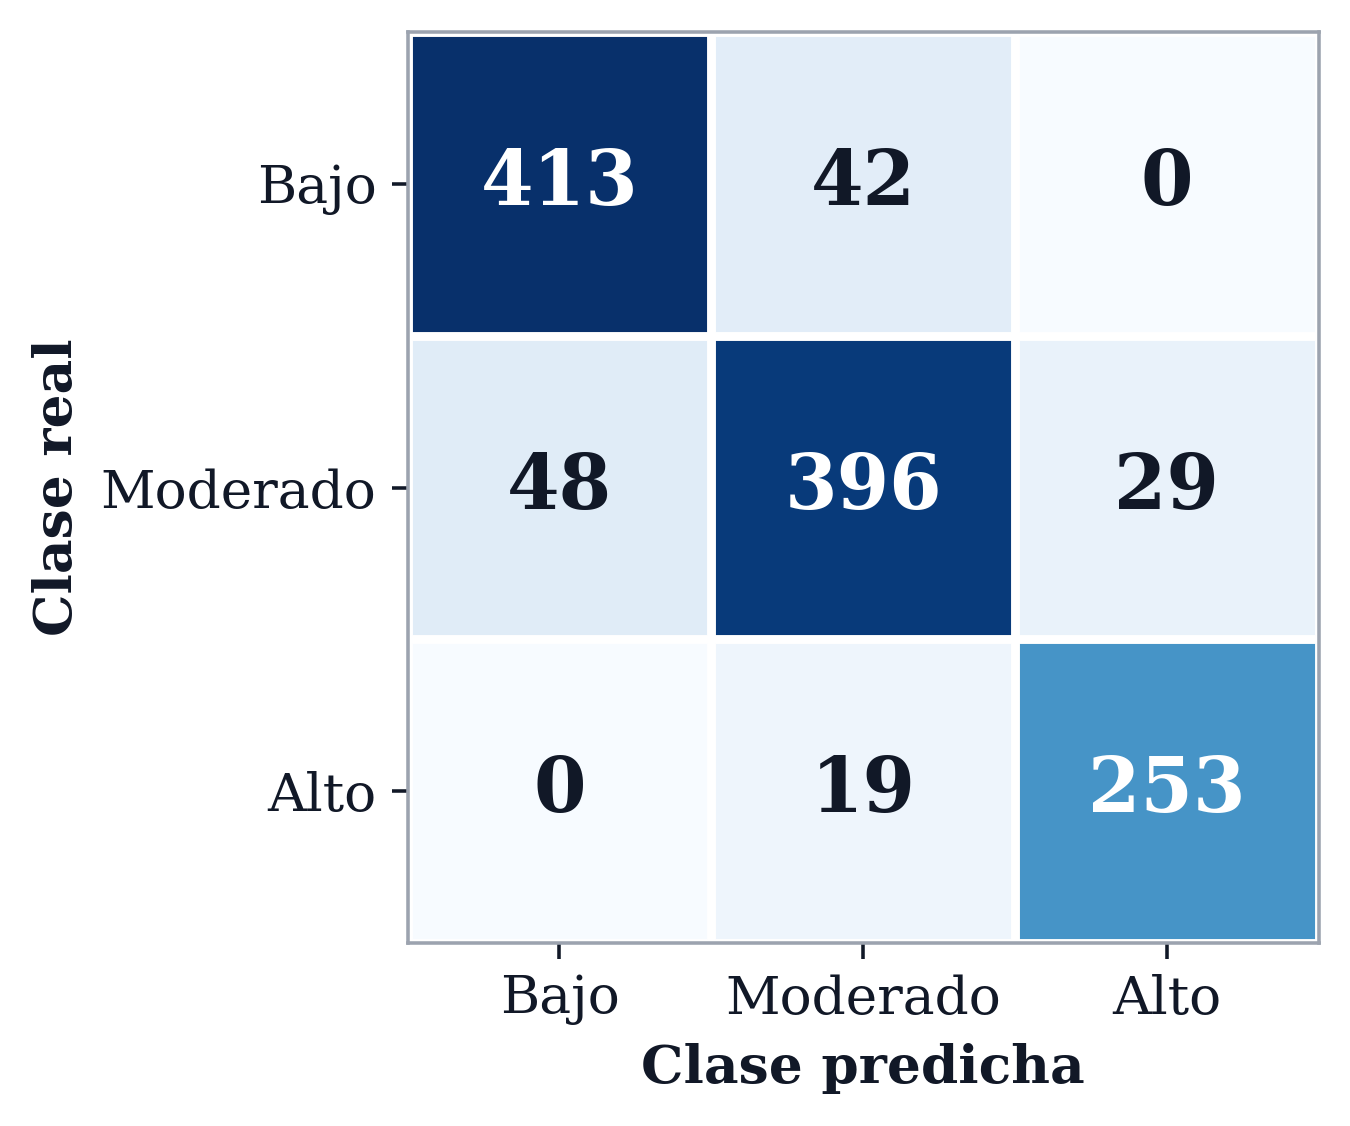
\includegraphics[width=0.92\textwidth]{fig_confusion.png}
\caption{Matrices de confusión del mejor modelo (\BestOpt{}) sobre el conjunto de prueba, un panel por
\textit{target}.}
\label{fig:conf}
\end{figure*}

\subsection{C9. Diagnóstico de sobreaprendizaje}
\label{sec:c9}
¿Es el problema propenso al sobreaprendizaje? La evidencia es cuantitativa. Cuando se libera la profundidad
del \textit{random forest}, el F1-macro en entrenamiento alcanza \LCtrainEnd{} mientras que en validación se
estanca en \LCcvEnd{}: una brecha de \LCgap{} (Figura~\ref{fig:lc}). Esa diferencia es la firma del
sobreaprendizaje: el modelo memoriza el ruido (\texttt{flip\_y=0.02}) y las particiones espurias de las
variables redundantes. La curva también muestra que la brecha se reduce al aumentar el tamaño de la muestra,
lo que indica que \emph{más datos} y \emph{menor capacidad} son las palancas correctas.

\begin{figure}[H]
\centering
\includegraphics[width=\columnwidth]{fig_learning_curve.png}
\caption{Curva de aprendizaje del mejor modelo. La separación persistente entre entrenamiento y validación
revela sobreaprendizaje; la brecha decrece con más datos.}
\label{fig:lc}
\end{figure}

El análisis de PCA (Figura~\ref{fig:pca}) refuerza el diagnóstico: bastan \PCAneff{} de los \Nfeatures{}
componentes para explicar el 95\% de la varianza, señal de redundancia entre atributos que un modelo de
alta capacidad puede sobreajustar.

\begin{figure}[H]
\centering
\includegraphics[width=0.86\columnwidth]{fig_pca_variance.png}
\caption{Varianza explicada acumulada por PCA. Con \PCAneff{} componentes se alcanza el 95\%.}
\label{fig:pca}
\end{figure}

%==========================================================
% 7. CONCLUSIONES
%==========================================================
\section{Conclusiones}
Las conclusiones se expresan como métricas, no como opiniones.
\begin{itemize}[leftmargin=1.1em,itemsep=2pt]
\item \textbf{Sobre O3--O4 (optimización).} Los optimizadores que buscan también sobre la elección del
algoritmo dominaron: el genético alcanzó el mayor F1-macro en prueba (\GenFtest{}) y Optuna lo igualó
prácticamente (\OptunaFtest{}, diferencia de apenas 0.0006) en menos tiempo (\OptunaTime{}~s frente a
\GenTime{}~s). Ambos superaron por más de 6 puntos a la cuadrícula (\GridFtest{}, \GridTime{}~s) y a la
búsqueda aleatoria (\RandFtest{}, \RandTime{}~s), que quedaron ancladas a \textit{random forest}. La
optimización bayesiana es, por tanto, la más eficiente (mejor calidad por unidad de tiempo).
\item \textbf{Sobre el algoritmo de aprendizaje.} Entre los cinco algoritmos, \BestAlgo{} obtuvo el mayor
F1-macro en validación (\BestAlgoF{}) y \WorstAlgo{} el menor (\WorstAlgoF{}); la elección del algoritmo
(diferencia de \BestAlgoF{} vs \WorstAlgoF{}) pesa más que el ajuste fino de un único modelo, lo que explica
por qué Grid y Random ---fijados a \textit{random forest}--- no alcanzaron el tope.
\item \textbf{Sobre el objetivo general (minimizar el error).} El mejor procedimiento alcanzó una
\textit{Hamming loss} de \OptunaHam{} y una \textit{subset accuracy} de \OptunaSubset{} sobre \Ntest{}
registros de prueba nunca vistos.
\item \textbf{Sobre el sobreaprendizaje.} El problema es propenso a él: la brecha entrenamiento--validación
llega a \LCgap{} con capacidad alta, y se atenúa con más datos y regularización.
\item \textbf{Sobre el costo.} El tiempo total de las cuatro búsquedas fue de \TotalRuntime{}~s sobre
\Searchsub{} registros, lo que vuelve viable repetir la optimización en cada ciclo de reentrenamiento.
\end{itemize}

%==========================================================
% 8. RECOMENDACIONES
%==========================================================
\section{Recomendaciones}
Se proponen y se \emph{implementan} tres recomendaciones; su viabilidad se decide por métrica
(Tabla~\ref{tab:rec}, Figura~\ref{fig:rec}).
\begin{enumerate}[leftmargin=1.2em,itemsep=2pt]
\item \textbf{Ponderar las clases} (\texttt{class\_weight=balanced}) para atacar el desbalanceo. Resultado:
F1-macro \RecOneF{} (\RecOneDelta{} sobre la línea base) sin costo de preprocesamiento adicional.
\textbf{\RecOneViable{}}.
\item \textbf{Reducir dimensionalidad con PCA al 95\%} (\RecTwoComp{} componentes) para acelerar la
inferencia. Resultado: F1-macro \RecTwoF{} (\RecTwoDelta{}); intercambia algo de calidad por velocidad,
por lo que resulta \textbf{\RecTwoViable{}} bajo el criterio adoptado.
\item \textbf{Aumentar la capacidad del modelo} (más árboles y mayor profundidad). Resultado: F1-macro
\RecThreeF{} (\RecThreeDelta{}); el beneficio marginal no compensa el mayor costo y riesgo de
sobreaprendizaje, por lo que es \textbf{\RecThreeViable{}}.
\end{enumerate}

\begin{table}[H]
\centering
\caption{Recomendaciones implementadas y su impacto frente a la línea base.}
\label{tab:rec}
\small
\begin{tabularx}{\columnwidth}{Xcccc}
\toprule
\textbf{Propuesta} & \textbf{F1 test} & \textbf{Brecha} & \textbf{t (s)} & \textbf{Viable} \\
\midrule
\TablaRec
\bottomrule
\end{tabularx}
\end{table}

\begin{figure}[H]
\centering
\includegraphics[width=\columnwidth]{fig_recommendations.png}
\caption{Impacto de cada recomendación en calidad (izq.) y costo de ajuste (der.) respecto de la línea
base (línea discontinua).}
\label{fig:rec}
\end{figure}

\noindent En síntesis, solo la primera recomendación es plenamente viable: mejora la métrica atacando la
causa raíz (el desbalanceo) sin penalización de costo.

%==========================================================
% REFERENCIAS
%==========================================================
\begin{thebibliography}{99}
\small
\bibitem{breiman2001} L. Breiman, ``Random Forests,'' \textit{Machine Learning}, vol.~45, no.~1,
pp.~5--32, 2001. DOI: 10.1023/A:1010933404324.
\bibitem{bergstra2012} J. Bergstra and Y. Bengio, ``Random Search for Hyper-Parameter Optimization,''
\textit{Journal of Machine Learning Research}, vol.~13, pp.~281--305, 2012. DOI: 10.5555/2188385.2188395.
\bibitem{shahriari2016} B. Shahriari, K. Swersky, Z. Wang, R.~P. Adams, and N. de Freitas, ``Taking the
Human Out of the Loop: A Review of Bayesian Optimization,'' \textit{Proceedings of the IEEE}, vol.~104,
no.~1, pp.~148--175, 2016. DOI: 10.1109/JPROC.2015.2494218.
\bibitem{akiba2019} T. Akiba, S. Sano, T. Yanase, T. Ohta, and M. Koyama, ``Optuna: A Next-generation
Hyperparameter Optimization Framework,'' in \textit{Proc. 25th ACM SIGKDD Int. Conf. on Knowledge Discovery
\& Data Mining}, 2019, pp.~2623--2631. DOI: 10.1145/3292500.3330701.
\bibitem{feurer2019} M. Feurer and F. Hutter, ``Hyperparameter Optimization,'' in \textit{Automated Machine
Learning}, Springer, 2019, pp.~3--33. DOI: 10.1007/978-3-030-05318-5\_1.
\bibitem{goldberg1989} D.~E. Goldberg, \textit{Genetic Algorithms in Search, Optimization, and Machine
Learning}. Addison-Wesley, 1989. ISBN: 978-0201157673.
\bibitem{tsoumakas2007} G. Tsoumakas and I. Katakis, ``Multi-Label Classification: An Overview,''
\textit{International Journal of Data Warehousing and Mining}, vol.~3, no.~3, pp.~1--13, 2007.
DOI: 10.4018/jdwm.2007070101.
\bibitem{read2011} J. Read, B. Pfahringer, G. Holmes, and E. Frank, ``Classifier Chains for Multi-label
Classification,'' \textit{Machine Learning}, vol.~85, no.~3, pp.~333--359, 2011.
DOI: 10.1007/s10994-011-5256-5.
\bibitem{pearson1901} K. Pearson, ``On Lines and Planes of Closest Fit to Systems of Points in Space,''
\textit{Philosophical Magazine}, vol.~2, no.~11, pp.~559--572, 1901. DOI: 10.1080/14786440109462720.
\bibitem{hastie2009} T. Hastie, R. Tibshirani, and J. Friedman, \textit{The Elements of Statistical
Learning}, 2nd ed. Springer, 2009. ISBN: 978-0387848570.
\bibitem{geron2019} A. Géron, \textit{Hands-On Machine Learning with Scikit-Learn, Keras, and
TensorFlow}, 2nd ed. O'Reilly, 2019. ISBN: 978-1492032649.
\end{thebibliography}

\end{document}
